\documentclass[a4paper,fleqn]{cas-dc}

\usepackage[numbers]{natbib}
\usepackage{amsmath, amsfonts, amssymb}
\usepackage{algorithm, algpseudocode}
\usepackage{graphicx}
\usepackage{adjustbox}
\usepackage{booktabs, tabularx, multirow}
\usepackage{enumitem}
\usepackage{ragged2e}
\usepackage{microtype}
\usepackage{float}
\usepackage{xcolor}
\definecolor{revisiongreen}{RGB}{0,100,0}
\colorlet{green}{revisiongreen}
\definecolor{revisionpurple}{HTML}{6A0DAD}
\colorlet{purple}{revisionpurple}
\definecolor{revisionorange}{HTML}{B35A00}
\definecolor{revisionbrown}{HTML}{6B3A2A}
\setlist{nosep}

\hypersetup{hypertexnames=false}

\widowpenalty=10000
\clubpenalty=10000
\emergencystretch=3em
\hfuzz=130pt

\makeatletter
\g@addto@macro\UrlBreaks{\do\.\do\@\do\-\do\_}
\makeatother

\newcommand*\D{\mathop{}\!\mathrm{d}}
\DeclareMathOperator{\sg}{sg}

\begin{document}

\shorttitle{Pricing Swing Options in Energy Markets using DRL}

\title[mode=title]{\texorpdfstring{Pricing Swing Options in Energy Markets\\using Deep Reinforcement Learning}{Pricing Swing Options in Energy Markets using Deep Reinforcement Learning}}

\author[1]{Alexander Tsoskounoglou}[]
\ead{alexander.tsoskounoglou@gmail.com}

\author[2,3]{Sven Karbach}[]
\ead{sven@karbach.org}

\author[2,3]{Konstantinos Chatziandreou}[]
\ead{k.chatziandreou@uva.nl}

\affiliation[1]{%
    organization={Morgan Stanley},
    city={Budapest},
    country={Hungary}
}

\affiliation[2]{%
    organization={Informatics Institute, University of Amsterdam},
    city={Amsterdam},
    country={The Netherlands}
}

\affiliation[3]{%
    organization={Korteweg-de Vries Institute, University of Amsterdam},
    city={Amsterdam},
    country={The Netherlands}
}

\begin{abstract}
    We study the valuation of electricity swing options under spot dynamics with seasonality, mean reversion, and spikes. Prices follow the Hambly--Howison--Kluge (HHK) model, and the contract is cast as a finite-horizon stochastic control problem with continuous exercise quantities, a cumulative volume cap, and convex exercise costs. We propose a deterministic actor--critic method whose profitability-gated actor clips candidate exercises to quantities with non-negative immediate payoff while preserving gradient flow via a straight-through estimator. The method avoids explicit state-space discretisation and works with a nine-dimensional Markov state that combines market factors with contract bookkeeping variables. \textcolor{revisionbrown}{Numerical experiments against a discretized-action least-squares Monte Carlo baseline show that the two methods produce comparable option values: the LSM baseline is generally competitive, while the actor--critic approach narrows the gap and occasionally prevails in configurations where strong cost convexity makes fine-grained exercise modulation most valuable.}
\end{abstract}

\begin{keywords}
    Deep reinforcement learning \sep Swing options \sep HHK model \sep
    Convex exercise costs \sep Actor--critic methods
\end{keywords}

\sloppy
\maketitle
\fussy

\ExplSyntaxOn
\cs_gset:Npn \__first_footerline:
{
    \group_begin:
    \small
    \sffamily
    \ifnum \theblind > 0 \relax
    \else
        \texttt{\MakeLowercase{Contact:}}~%
        {\rmfamily\itshape
            \texttt{\MakeLowercase{alexander.tsoskounoglou@gmail.com}}%
        }%
    \fi
    \group_end:
}
\ExplSyntaxOff

\section{Introduction}
\label{sec:introduction}

Electricity markets display several features that distinguish them from traditional financial markets: non-storability, strong seasonality, abrupt demand--supply imbalances, and short-lived price spikes. A substantial literature therefore models electricity prices using mean-reverting diffusions augmented by jump components. Early two-factor Gaussian models were introduced by~\cite{lucia2002electricity}, while~\cite{cartea2005pricing} incorporated jumps to capture extreme movements. A major refinement was provided by~\cite{Hambly2009}, who specified the log spot price as the sum of a seasonal component, an Ornstein--Uhlenbeck factor, and a rapidly mean-reverting spike factor. The resulting model captures both ordinary price fluctuations and transient spikes while remaining tractable enough for calibration and valuation.

Swing options are central in gas and power markets because they grant the holder repeated rights to purchase energy subject to volume and operational constraints. Their valuation is substantially more involved than that of European-style derivatives, since the holder repeatedly decides how much to exercise at each decision time. Classical approaches include tree and grid-based dynamic programming~\cite{jaillet2004valuation}, Monte Carlo regression methods~\cite{longstaff2001valuing,meinshausen2004monte}, dual or multiple-stopping formulations~\cite{carmona2008swing}, and analytically tractable special cases. These methods can be accurate, but they become increasingly cumbersome when the underlying model contains multiple stochastic factors, jump components, and non-trivial contractual constraints.

Reinforcement learning and neuro-dynamic programming provide an attractive alternative to explicit state-space discretisation~\cite{bertsekas1996neuro,sutton1998reinforcement}. \textcolor{green}{Recent financial applications include deep hedging, optimal stopping, and related control problems~\cite{halperin2017qlbs,buehler2019deephedging,becker2019deepoptimalstopping,tsoskounoglou2025higherorder}.} Swing contracts are a natural testbed: the exercise decision is continuous, the horizon is finite but non-trivial, and the contract state embeds directly into the Markov state observed by the agent.

In this paper we formulate swing-option valuation under the HHK model as a finite-horizon Markov decision process and solve the resulting control problem with a deterministic actor--critic algorithm. The focus is on contracts with optional exercise, a cumulative volume cap, and convex exercise costs, since convexity destroys the bang-bang structure that simplifies many classical implementations. Our main contributions are:
\begin{enumerate}
    \item a \textbf{profitability-gated actor} that clips proposed exercises to quantities with non-negative immediate payoff while preserving gradient flow through a straight-through estimator;
    \item a \textbf{nine-dimensional state representation} that combines HHK market factors with contract bookkeeping variables in a Markovian input to the policy and value networks;
    \item a \textbf{deterministic actor--critic training procedure} with prioritized replay, target smoothing, and pre-squash exploration noise tailored to continuous exercise decisions; and
    \item a set of \textbf{numerical experiments} showing how the learned policy compares with a \textcolor{revisionbrown}{discretized-action} LSM baseline across a range of convex cost specifications.
\end{enumerate}

The remainder of the paper is organised as follows. Section~\ref{sec:market_contract} introduces the HHK price model and the swing-contract specification used throughout the manuscript. Section~\ref{sec:classical_methods} summarises the classical dynamic-programming perspective that motivates the reinforcement-learning approach. Section~\ref{sec:rl_formulation} presents the Markov decision process, actor--critic architecture, and profitability gate. Section~\ref{sec:experiments} reports numerical results, and Section~\ref{sec:conclusion} concludes.

\section{Market and Contract Framework}
\label{sec:market_contract}

\subsection{Electricity Spot Price Dynamics: the HHK Model}

We model the electricity spot price directly under a pricing measure $\mathbb{Q}$ calibrated to observed forward prices. This is standard in reduced-form energy modelling: rather than deriving a unique martingale measure from storage-based no-arbitrage arguments, one specifies a tractable pricing dynamics consistent with traded forward curves; see~\cite{lucia2002electricity,cartea2005pricing,Hambly2009}. Let $(\Omega,\mathcal{F},(\mathcal{F}_t)_{t \ge 0},\mathbb{Q})$ be a filtered probability space supporting a Brownian motion $W$ and an independent Poisson process $N$ with intensity $\lambda$.

Following~\cite{Hambly2009}, the spot price is written as
\begin{equation}
    \label{eq:model}
    S_t = \exp\!\bigl(f(t) + X_t + Y_t\bigr),
\end{equation}
where $f$ is a deterministic seasonal function and the latent factors satisfy
\begin{align}
    \D X_t & = -\alpha X_t \,\D t + \sigma \,\D W_t, \label{eq:OU} \\
    \D Y_t & = -\beta Y_t \,\D t + J_t \,\D N_t. \label{eq:jumpOU}
\end{align}
Here $\alpha > 0$ is the mean-reversion rate of the diffusive factor $X$, $\beta > 0$ is the mean-reversion rate of the spike factor $Y$, and typically $\beta \gg \alpha$ so that spikes decay quickly. The jump sizes $(J_t)$ are i.i.d.\ and non-negative, taken to be exponentially distributed with mean $\mu_J > 0$, following~\cite{Hambly2009,cartea2005pricing}. Restricting jumps to be positive models the empirical observation that electricity price spikes are predominantly upward.

The deterministic term $f(t)$ captures predictable seasonality in demand and supply. A simple illustration is
\[
    f(t) = \log(S_0) + A \cos(2 \pi t),
\]
although in practice one can use richer parametrisations. In the numerical experiments of Section~\ref{sec:experiments} we set $A = 0$, so that $f(t) = \log S_0$ and the seasonal component is flat. Under~\eqref{eq:model}--\eqref{eq:jumpOU}, the pair $(X_t,Y_t)$ is Markov and the distributional quantities needed for forward-curve fitting can be expressed semi-analytically; see~\cite{Hambly2009}. In particular, one may recover the seasonal component so that the model matches observed forwards via
\[
    F_t^{[T]} = \mathbb{E}^{\mathbb{Q}}[S_T \mid \mathcal{F}_t].
\]
To ensure forward-curve consistency, $f$ must absorb a convexity correction arising from the variance of $X_T$ and the moment-generating function of $Y_T$ under $\mathbb{Q}$; details are given in~\cite{Hambly2009}.

% P2-7: Replace Sven's red comment with an explicit justification for flat seasonality.
The choice $A = 0$ is motivated by the short contract maturity of approximately one month used in the numerical experiments.
Over a horizon of $T \approx 0.083$ years ($\approx 22$ trading days), the deterministic seasonal component $A\cos(2\pi t)$ changes by at most $|A|\cdot 2\pi T \approx 0.5A$, which is negligible relative to the diffusive and jump volatility for realistic values of $A$.
Setting $A = 0$ therefore isolates the contribution of the stochastic factors $(X,Y)$ without confounding seasonal trends, and keeps the pricing problem well-suited to comparing RL with LSM on a well-understood benchmark.
For longer-maturity contracts or seasonal calibration studies, $A > 0$ can be activated without modifying the algorithm.

The HHK model provides an appealing compromise between realism and tractability. It captures the empirical features that matter most for electricity options, yet it already makes classical grid-based valuation demanding because the state space contains two latent factors and a jump component. This is precisely the regime in which simulation-based control methods become attractive.

\subsection{Swing Contract Specification}

We consider a finite set of exercise dates
\[
    0 = t_0 < t_1 < \cdots < t_{n-1} < t_n = T,
    \qquad
    t_i = i \Delta t,
\]
with a constant time step $\Delta t = T/n$. At each exercise date $t_i$, the holder chooses a non-negative quantity
\[
    q_i \in [0,q_{\max}],
\]
where $q_{\max}$ is the maximum offtake per exercise date. The cumulative exercised volume is tracked by
\[
    Q_0 = 0,
    \qquad
    Q_{i+1} = Q_i + q_i,
\]
and the contract imposes the cumulative cap
\[
    Q_n = \sum_{i=0}^{n-1} q_i \le Q_{\max}.
\]
Throughout the reported experiments, zero exercise is always admissible. This feature is important for both the economic interpretation and the profitability arguments used later.

\paragraph{Operational constraints.}
The framework also accommodates optional operational constraints. A refraction period of length $L \in \mathbb{N}_0$ requires the holder to wait $L$ exercise dates after any strictly positive exercise:
\[
    q_i > 0 \implies q_{i+1} = \cdots = q_{i+L} = 0,
\]
with the obvious truncation near maturity. Likewise, ramping constraints of the form
\[
    |q_{i+1} - q_i| \le R
\]
can be incorporated by augmenting the state. The numerical experiments in Section~\ref{sec:experiments} focus on the baseline case with zero refraction lag and no ramping constraints, but the notation below is chosen so that these features can be activated without changing the basic formulation.

\paragraph{Payoff with convex exercise costs.}
Let $K$ denote the contractual strike and let $\gamma_c \ge 1$ be the cost exponent. Exercising $q_i$ units at time $t_i$ yields
\begin{equation}
    \label{eq:payoff}
    \Pi_i(q_i) = q_i (S_{t_i} - K)^+ - c q_i^{\gamma_c},
\end{equation}
where $c \ge 0$ is the cost coefficient. The term $c q_i^{\gamma_c}$ may be interpreted as an imbalance charge, liquidity penalty, or reduced-form operational disutility. When $\gamma_c = 1$, the cost is linear and the immediate payoff is affine in $q_i$. When $\gamma_c > 1$, the cost is convex and interior optimal exercises can arise.

The use of the positive part $(S_{t_i} - K)^+$ makes the contract a \emph{call-like} swing option: exercising is purely optional and the holder never pays more than the cost component $c q_i^{\gamma_c}$. This distinguishes the present formulation from take-or-pay contracts in which the per-unit payoff is $S_{t_i} - K$ (which may be negative) and minimum-volume obligations effectively enforce exercise. Our optional-exercise assumption is natural for the profitability gate introduced in Section~\ref{sec:profitability_gate} and is standard in the financial options literature~\cite{jaillet2004valuation,carmona2008swing}.

\paragraph{Admissible controls and contract value.}
Let $\mathcal{A}_i(h_i)$ denote the set of feasible exercises at time $t_i$ given the current history $h_i$, including the per-period cap, remaining cumulative volume, and any active operational constraints. An admissible policy is a sequence of $\mathcal{F}_{t_i}$-measurable decisions $(q_i)_{i=0}^{n-1}$ with $q_i \in \mathcal{A}_i(h_i)$ almost surely. The time-zero value of the swing contract is then
\begin{equation}
    \label{eq:value0}
    V_0 = \sup_{(q_i) \in \mathcal{Q}}
    \mathbb{E}^{\mathbb{Q}}
    \biggl[
        \sum_{i=0}^{n-1} e^{-r t_i} \Pi_i(q_i)
        \biggr],
\end{equation}
where $\mathcal{Q}$ is the set of admissible policies and $r$ is the discount rate used under the chosen pricing measure. Since $t_i = i \Delta t$, it is convenient to write
\[
    \delta = e^{-r \Delta t},
    \qquad
    e^{-r t_i} = \delta^i.
\]
Equation~\eqref{eq:value0} is the finite-horizon stochastic control problem solved in the remainder of the paper.

\section{Classical Methods and Motivation}
\label{sec:classical_methods}

Before turning to reinforcement learning, it is useful to recall the classical dynamic-programming viewpoint for swing-option valuation under HHK dynamics. We do not implement the full HHK grid method in the numerical section below, but it provides the natural point of comparison for discussing the curse of dimensionality and motivates the simulation-based approach adopted later.

\subsection{Grid-Based Dynamic Programming}

Under the HHK model with contract bookkeeping variables, a Markov state can be written as
\[
    \begin{aligned}
        Z_i = \bigl( & X_{t_i},\,Y_{t_i},  \\
                     & Q_i,\,\rho_i\bigr),
    \end{aligned}
\]
where $\rho_i$ denotes any additional operational counter, for example the remaining refraction lag. A grid-based method approximates the continuous state space by structured grids
\[
    \begin{aligned}
        X_{t_i} & \in \{x_1,\dots,x_{N_X}\},       \\
        Y_{t_i} & \in \{y_1,\dots,y_{N_Y}\},       \\
        Q_i     & \in \{q^{(0)},\dots,q^{(N_Q)}\},
    \end{aligned}
\]
and, if required, a finite grid for the refraction state.

If the action set is also discretised, the grid Bellman recursion takes the form
\begin{equation}
    \label{eq:grid_bellman}
    V_i(z) = \max_{a \in \mathcal{A}_i(z)}
    \left[
        \Pi_i(a)
        + \delta \sum_{z'} P_i(z,z';a) V_{i+1}(z')
        \right],
\end{equation}
with terminal condition $V_n \equiv 0$. Here $P_i(z,z';a)$ denotes the one-step transition probability between neighbouring grid states, including both the latent-factor dynamics and the contract bookkeeping update. The diffusion factor $X$ admits an exact Gaussian transition, while the spike factor $Y$ leads to a Poisson mixture that must be approximated numerically~\cite{Hambly2009}.

\subsection{Why Continuous-Control RL is Attractive}

Even in the baseline HHK setting, classical methods face several structural difficulties:
\begin{itemize}
    \item \textbf{State dimensionality.} The latent factors $(X,Y)$ already require a two-dimensional grid before contract variables are added.
    \item \textbf{Jump dynamics.} Accurate treatment of the spike component requires either a fine grid or careful approximation of the jump mixture.
    \item \textbf{Continuous actions.} The true control is continuous on $[0,q_{\max}]$, so grid methods must discretise the action space and thereby introduce an additional approximation.
    \item \textbf{Convex costs.} When $\gamma_c > 1$, interior exercises are possible and the bang-bang simplifications used in some classical implementations no longer apply.
\end{itemize}

These issues motivate a simulation-based method that works with continuous actions and sampled trajectories rather than transition densities on a grid. The reinforcement-learning formulation developed next is designed for exactly this setting.

\section{Reinforcement Learning Formulation}
\label{sec:rl_formulation}

We now cast~\eqref{eq:value0} as a finite-horizon Markov decision process. The objective remains the discounted contract value under $\mathbb{Q}$; reinforcement learning enters only as a numerical method for approximating the optimal control.

\subsection{Markov Decision Process}
\label{sec:mdp}

At exercise time $t_i$, the agent observes a nine-dimensional state
\[
    \begin{aligned}
        s_i = \bigl( & S_{t_i} - K,
        Q_i / Q_{\max},
        (Q_{\max} - Q_i) / Q_{\max}, \\
                     & (T - t_i)/T,
        i/n,
        S_{t_i},
        X_{t_i},
        Y_{t_i},
        \rho_i\bigr).
    \end{aligned}
\]
The display above lists the raw economic quantities; Table~\ref{tab:state_components} details the meaning and preprocessing applied to each component before network ingestion (e.g., log-moneyness and robust scaling). The state contains all variables required to make the problem Markov. \textcolor{purple}{The representation is intentionally non-minimal: the paired inventory features $Q_i/Q_{\max}$ and $(Q_{\max}-Q_i)/Q_{\max}$, as well as the paired time features $(T-t_i)/T$ and $i/n$, encode the same information up to affine transforms. We retain both pairs as an engineering choice because they stabilised optimisation in our experiments. This is consistent with the broader DRL hedging literature, where state design is largely task-specific and recent reviews report no consensus minimal representation, with practical implementations often preferring richer feature sets over theoretically minimal ones \cite{kolm2019dynamic,pickard2023review,cao2022gamma}. A systematic minimal-state ablation is left for future work.} \textcolor{red}{\textbf{Sven:} While noted as practically useful, the inclusion of redundant state variables ($Q_i/Q_{\max}$ vs $(Q_{\max}-Q_i)/Q_{\max}$, and $t_i$ vs $i/n$) is theoretically not super elegant. Worth it to reduce to a minimal sufficient basis to strengthen the theoretical presentation?}

\begin{table}[htbp]
    \centering
    \caption{State representation for the swing-option MDP.}
    \label{tab:state_components}
    \begin{adjustbox}{max width=\linewidth}
        \begin{tabular}{clll}
            \toprule
            Index & Symbol                      & Description                          & Transformation                  \\
            \midrule
            0     & $S_{t_i} - K$               & Intrinsic spread                     & Raw                             \\
            1     & $Q_i / Q_{\max}$            & Used-volume fraction                 & $[0,1]$                         \\
            2     & $(Q_{\max} - Q_i)/Q_{\max}$ & Remaining-volume fraction            & $[0,1]$                         \\
            3     & $(T - t_i)/T$               & Time to maturity                     & $[0,1]$                         \\
            4     & $i/n$                       & Contract progress                    & $[0,1]$                         \\
            5     & $S_{t_i}$                   & Spot price                           & Log-moneyness $\log(S_{t_i}/K)$ \\
            6     & $X_{t_i}$                   & Diffusive factor                     & Robust-scaled (median/IQR)      \\
            7     & $Y_{t_i}$                   & Spike factor                         & Robust-scaled (median/IQR)      \\
            8     & $\rho_i$                    & Normalised steps since last exercise & $[0,1]$                         \\
            \bottomrule
        \end{tabular}
    \end{adjustbox}
\end{table}

The actor outputs a normalised exercise
\[
    \tilde{q}_i \in [0,1],
\]
which is mapped to the physical exercise quantity by
\[
    q_i = q_{\max} \tilde{q}_i.
\]
The environment then clips this proposal to the remaining capacity:
\[
    q_i \leftarrow \min\{q_i, Q_{\max} - Q_i\}.
\]
The next state is obtained by advancing the HHK simulator over one exercise interval and updating the contract bookkeeping variables,
\[
    \begin{aligned}
        \bigl(X_{t_{i+1}},Y_{t_{i+1}}\bigr)
                & = \operatorname{SimHHK}\bigl(X_{t_i},Y_{t_i};\Delta t\bigr), \\
        Q_{i+1} & = Q_i + q_i.
    \end{aligned}
\]
We write $\operatorname{SimHHK}$ for the one-step simulation routine used on the exercise grid; it draws from the exact conditional distributions of $X$ and $Y$ under $\mathbb{Q}$. The presentation below does not rely on a particular discretisation scheme, only on the ability to simulate the model consistently under the pricing measure.

% P2-6: Document Sobol QMC for OU increments and antithetic variates for jump component.
\paragraph{Variance reduction in path generation.}
The implementation uses two variance-reduction techniques when generating the training and evaluation paths.
For the Ornstein--Uhlenbeck diffusion component $X$, the Brownian increments $\Delta W \sim \mathcal{N}(0,\Delta t)$ are drawn via a scrambled Sobol quasi-Monte Carlo sequence (dimension equal to $n \times N_{\mathrm{paths}}$), improving the uniformity of path coverage relative to plain pseudo-random sampling.
For the compound Poisson jump component $Y$, antithetic variates are applied: each path is paired with a mirror path that uses the negative of its Poisson arrivals and jump sizes, so that the estimator averages out the first-order sampling error from the jump noise.
These techniques reduce the variance of the option-price estimator at fixed path count and are particularly beneficial for the evaluation step, which uses $65{,}536$ held-out paths.

The one-step reward is the undiscounted exercise payoff
\[
    R_i(q_i) = \Pi_i(q_i),
\]
and the objective is
\[
    J(\pi) =
    \mathbb{E}^{\mathbb{Q}}
    \biggl[
        \sum_{i=0}^{n-1} \delta^i R_i(q_i)
        \biggr].
\]
This is exactly the swing-option value~\eqref{eq:value0} for the policy class represented by the actor. Note that the RL discount factor $\delta = e^{-r\Delta t}$ coincides with the financial discount factor in the pricing objective, and all paths are simulated under the risk-neutral measure $\mathbb{Q}$, so the RL and derivative-pricing problems are formally identical.

\paragraph{Implementation note (pre-discounted reward convention).}
% P1-8: Document that the implementation uses pre-discounted rewards with GAMMA=1.
In the implementation, the one-step reward stored in the replay buffer is the \emph{pre-discounted} payoff $\tilde R_i = \delta^i \Pi_i(q_i)$, and the Bellman target is computed with RL discount factor $\gamma_{\mathrm{RL}} = 1$.
This is equivalent to the formulation above: the Bellman recursion with $\gamma_{\mathrm{RL}} = 1$ and pre-discounted rewards reconstructs the same sum $\sum_i \delta^i \Pi_i(q_i)$ as a standard $\gamma_{\mathrm{RL}} = \delta$ recursion with undiscounted rewards.
The pre-discounted convention avoids introducing a second discount mechanism in the critic loss, and is reflected in the hyperparameter $\gamma = 1$ listed in Table~\ref{tab:hyperparams}.

\subsection{Enforcement of Swing Constraints}

The contract constraints enter the RL formulation through the environment and the action post-processing.

\paragraph{Per-period cap and cumulative cap.}
The actor proposes a normalised action in $[0,1]$, which corresponds to a physical exercise in $[0,q_{\max}]$. The environment then enforces the cumulative cap by clipping to the remaining capacity $Q_{\max} - Q_i$.

\paragraph{Refraction constraints.}
% P2-1: rho_i is implemented as normalised steps since last exercise, not remaining blocked fraction.
\textcolor{purple}{The state variable $\rho_i$, taking values in $[0,1]$, records the normalised number of steps elapsed since the last exercise and acts as a soft proximity signal for refraction-style constraints.}

\textcolor{purple}{If a mandatory refraction period is active, the environment forces $q_i = 0$ while a cooldown counter is positive. Then $\rho_i$ gives the policy a continuous summary of how recently the last exercise occurred. In the reported experiments no refraction is imposed, so $\rho_i$ carries elapsed-since-exercise information only. Retaining it in the state nevertheless makes the extension to richer contracts explicit.}

\paragraph{Profitability masking.}
\textcolor{purple}{For the contract class studied numerically, zero exercise is always admissible and only an upper cumulative volume cap is imposed. Consequently, any action with strictly negative immediate payoff is weakly dominated by zero exercise: it lowers the current cash flow and consumes flexibility that could be used later. This observation justifies the profitability gate introduced in Section~\ref{sec:profitability_gate}. We do not claim the same argument without modification for contracts with mandatory take obligations, active ramping constraints, or hard refraction limits. Under such path-dependent restrictions, it may be optimal to accept a small immediate loss in order to preserve feasibility for a more valuable future exercise, so the hard gate would need to be relaxed.}

\subsection{Actor--Critic Algorithm}
\label{sec:actor_critic}

We use a deterministic actor--critic architecture~\cite{silver2014dpg}, inspired by the distributed D4PG framework of~\cite{barth2018d4pg}, with target networks, prioritized experience replay (PER), and target-policy smoothing. The actor $\pi_\theta : \mathcal{S} \to [0,1]$ maps states to normalised exercise quantities, while the critic $Q_\phi : \mathcal{S} \times \mathcal{A} \to \mathbb{R}$ estimates discounted continuation values.

\subsubsection{Deterministic Policy Gradient}

The actor is trained by ascending the critic value~\cite{silver2014dpg},
\[
    \nabla_\theta J(\theta)
    =
    \mathbb{E}_{s \sim \mathcal{D}}
    \left[
        \nabla_a Q_\phi(s,a)\big|_{a=\pi_\theta(s)}
        \nabla_\theta \pi_\theta(s)
        \right],
\]
where $\mathcal{D}$ denotes the replay buffer. Target networks $(\pi_{\theta'},Q_{\phi'})$ are updated by Polyak averaging,
\[
    \theta' \leftarrow (1-\tau)\theta' + \tau \theta,
    \qquad
    \phi' \leftarrow (1-\tau)\phi' + \tau \phi,
\]
with $\tau = 0.0032$.

\subsubsection{Critic Loss}

The critic is scalar-valued and is trained with the one-step temporal-difference target
\[
    y = R + \delta (1-d) Q_{\phi'}\bigl(s',\pi_{\theta'}(s')\bigr),
\]
where $d$ is the terminal indicator and $R$ is the one-step reward. The loss is
\begin{equation*}
    \mathcal{L}_{\mathrm{critic}}
    =
    \mathbb{E}_{(s,a,R,s',d) \sim \mathcal{D}}
    \Bigl[
        w_i \bigl(y - Q_\phi(s,a)\bigr)^2
        \Bigr],
\end{equation*}
with importance-sampling weights $w_i$ supplied by PER.

\subsubsection{Prioritized Replay}

Transition $i$ is sampled with probability
\[
    P(i) = \frac{p_i^{a_{\mathrm{per}}}}{\sum_k p_k^{a_{\mathrm{per}}}},
    \qquad
    p_i = |\varepsilon_i| + \epsilon_{\mathrm{per}},
\]
where $\varepsilon_i$ is the TD error and $\epsilon_{\mathrm{per}} = 5 \times 10^{-6}$ is the priority floor. The priority exponent is annealed from $a_{\mathrm{per}} = 0.1$ to $0.2$. Importance weights use the exponent $b_{\mathrm{per}} = 1.0$:
\[
    w_i = (N P(i))^{-b_{\mathrm{per}}}.
\]
Renaming these replay exponents avoids confusion with the HHK parameters $\alpha$ and $\beta$.

\subsection{Profitability-Gated Actor}
\label{sec:profitability_gate}

Convex exercise costs imply that large exercises can be locally or globally unattractive even when the option is in the money. The actor therefore includes a hard gate that clips proposed exercises to quantities with non-negative immediate payoff.

\subsubsection{Profitability Region}

Fix a time $t_i$ and write
\[
    h_i = (S_{t_i} - K)^+.
\]
Then the immediate payoff is
\[
    \Pi_i(q) = h_i q - c q^{\gamma_c}.
\]
When $c > 0$ and $\gamma_c > 1$, the largest exercise that still yields non-negative immediate payoff is obtained from
\[
    h_i q = c q^{\gamma_c},
\]
namely
\begin{equation}
    \label{eq:qbar}
    \bar{q}_i =
    \left(
    \frac{h_i}{c}
    \right)^{1/(\gamma_c - 1)}.
\end{equation}
Therefore $\Pi_i(q) \ge 0$ for every $q \in [0,\bar{q}_i]$ and $\Pi_i(q) < 0$ for every $q > \bar{q}_i$. The stationary point of the immediate payoff is
\[
    q_i^{\mathrm{stat}} =
    \left(
    \frac{h_i}{c \gamma_c}
    \right)^{1/(\gamma_c - 1)},
\]
which lies below $\bar{q}_i$ and explains why interior optima arise under convex costs. The gate uses the zero-profit threshold $\bar{q}_i$, not the stationary point.

\subsubsection{Hard Gate Mechanism}

Let $\tilde{q}_i \in [0,1]$ be the raw actor output. The profitability gate clips it to
\[
    \tilde{q}_i^{\mathrm{gate}} =
    \min\!\left(
    \tilde{q}_i,
    \frac{\bar{q}_i}{q_{\max}},
    1
    \right)
\]
when $c > 0$ and $\gamma_c > 1$. For linear costs ($\gamma_c = 1$), the immediate payoff is affine in $q$ and non-negative exercise is possible only when $h_i \ge c$; otherwise the gate sets the action to zero.

\subsubsection{Straight-Through Estimator}

The clipping operation is non-differentiable, so we use a straight-through estimator:
\[
    \tilde{q}_i^{\mathrm{out}}
    =
    \tilde{q}_i + \sg\!\left(\tilde{q}_i^{\mathrm{gate}} - \tilde{q}_i\right).
\]
In the forward pass, $\tilde{q}_i^{\mathrm{out}} = \tilde{q}_i^{\mathrm{gate}}$; in the backward pass, gradients flow through the unclipped proposal $\tilde{q}_i$~\cite{bengio2013ste}. This retains a simple differentiable training signal while ensuring that the executed action satisfies the profitability bound. The STE introduces a biased gradient estimator; however, the bias is mild in practice because the gate is inactive for most training transitions (the actor quickly learns to avoid unprofitable exercises).

\subsubsection{Implementation}

Algorithm~\ref{alg:profitability_gate} summarises the gated actor forward pass.

\begin{algorithm}[htbp]
    \caption{Profitability-gated actor forward pass}
    \label{alg:profitability_gate}
    \begin{algorithmic}[1]
        \Require State $s_i$ with $(S_{t_i} - K)$ at index $0$
        \Require Cost parameters $c$, $\gamma_c$, $q_{\max}$
        \Ensure Feasible normalised action $\tilde{q}_i^{\mathrm{out}} \in [0,1]$
        \State $u \gets \operatorname{MLP}(s_i)$
        \State $\tilde{q}_i \gets \operatorname{sig}(\beta_{\mathrm{act}} u)$ \Comment{$\beta_{\mathrm{act}}$-sigmoid, $\beta_{\mathrm{act}} = 3.0$}
        \If{$c > 0$ and $\gamma_c > 1$}
        \State $\bar{q}_i \gets \bigl((S_{t_i}-K)^+/c\bigr)^{1/(\gamma_c-1)}$
        \State $\tilde{q}_i^{\max} \gets \min\{1,\bar{q}_i/q_{\max}\}$
        \State $\tilde{q}_i^{\mathrm{gate}} \gets \min\{\tilde{q}_i,\tilde{q}_i^{\max}\}$
        \ElsIf{$c > 0$ and $\gamma_c = 1$ and $(S_{t_i}-K)^+ < c$}
        \State $\tilde{q}_i^{\mathrm{gate}} \gets 0$
        \Else
        \State $\tilde{q}_i^{\mathrm{gate}} \gets \tilde{q}_i$
        \EndIf
        \State \Return $\tilde{q}_i + \sg(\tilde{q}_i^{\mathrm{gate}} - \tilde{q}_i)$
    \end{algorithmic}
\end{algorithm}

\subsection{Exploration Strategy}
\label{sec:exploration}

Exploration is challenging in continuous action spaces because the actor output is squashed to $[0,1]$. We therefore inject Gaussian noise before the output nonlinearity:
\[
    u_i' = u_i + \sigma_{\mathrm{expl}} \epsilon_i,
    \qquad
    \epsilon_i \sim \mathcal{N}(0,1).
\]
Pre-squash noise remains effective even when the policy is close to the action bounds. The noise scale follows a plateau-then-decay schedule,
\[
    \sigma_{\mathrm{expl}}(e) =
    \begin{cases}
        \sigma_0, & e < e_{\mathrm{plateau}},   \\[0.3em]
        \sigma_{\mathrm{floor}} +
        \dfrac{\sigma_0 - \sigma_{\mathrm{floor}}}
        {1 + \dfrac{e-e_{\mathrm{plateau}}}{e_{\mathrm{plateau}}}},
                  & e \ge e_{\mathrm{plateau}},
    \end{cases}
\]
\textcolor{green}{The schedule starts at 1.30, decays no lower than 0.26, and only begins to decay after 3{,}200 episodes.} % P2-5: Clarify that adaptive noise scales the std of the *pre-squash* noise by (1 + 0.6*|u_i|),
% where u_i is the pre-activation logit (not the squashed action in [0,1]).
We additionally scale the pre-squash noise standard deviation adaptively as
\[
    \begin{aligned}
        \tilde\sigma_i
         & = \sigma_{\mathrm{expl}}(e)             \\
         & \quad \cdot \bigl(1 + 0.6\,|u_i|\bigr),
    \end{aligned}
\]
where $u_i$ is the pre-squash logit output by the actor before the $\beta$-sigmoid nonlinearity.
This increases the effective noise magnitude when the logit is large (i.e.\ the policy is saturated near the action bounds), where the sigmoid gradient is small and unscaled noise would have little effect on the squashed output.

During the first $1{,}024$ episodes, actor updates are frozen and only the critic is trained. This critic warmup stabilises the early training dynamics. To reduce target overestimation, target-policy smoothing is applied in the critic target by perturbing the target action with clipped Gaussian noise.

\subsection{Neural Network Architecture}
\label{sec:architecture}

Both actor and critic are lightweight multilayer perceptrons. Table~\ref{tab:network_arch} summarises the architecture.

\begin{table}[htbp]
    \centering
    \caption{Neural-network architecture for actor and critic.}
    \label{tab:network_arch}
    \begin{adjustbox}{max width=\linewidth}
        \begin{tabular}{lll}
            \toprule
            Component         & Actor                          & Critic                 \\
            \midrule
            Input dimension   & 9 (state)                      & 9 (state) + 1 (action) \\
            Hidden layers     & 2                              & 2                      \\
            Hidden units      & 64                             & 64                     \\
            Activation        & SiLU                           & SiLU                   \\
            Normalisation     & LayerNorm                      & LayerNorm              \\
            Output dimension  & 1                              & 1                      \\
            Output activation & $\beta_{\mathrm{act}}$-sigmoid & None                   \\
            \bottomrule
        \end{tabular}
    \end{adjustbox}
\end{table}

\textcolor{green}{The actor output uses $\operatorname{sig}(\beta_{\mathrm{act}} u)$ with $\beta_{\mathrm{act}} = 3.0$, where $\operatorname{sig}$ denotes the logistic sigmoid. State preprocessing is domain-specific: the spot component is mapped to log-moneyness $\log(S_{t_i}/K)$; the latent factors $X_{t_i}$, $Y_{t_i}$ are robust-scaled using the sample median and IQR.
    Hidden-layer weights are initialised orthogonally with gain $\sqrt{2}$. Output layers use a small uniform initialisation drawn from the interval $[-0.003,0.003]$.}

Training uses AdamW with separate learning rates and weight decay:
\begin{itemize}
    \item actor: $\eta_a = 1.6 \times 10^{-4}$ with weight decay $5 \times 10^{-5}$;
    \item critic: $\eta_c = 9.0 \times 10^{-5}$ with weight decay $1.2 \times 10^{-4}$.
\end{itemize}
Both learning rates follow a warmup over the first $1{,}024$ episodes followed by cosine decay to $20\%$ of their initial values over $40{,}000$ episodes.

\subsection{Training Procedure}
\label{sec:training}

Algorithm~\ref{alg:training} gives the training loop.

\begin{algorithm}[htbp]
    \caption{Actor--critic training for swing-option pricing}
    \label{alg:training}
    \begin{algorithmic}[1]
        \Require Swing contract $\mathcal{C}$, HHK parameters $\Theta_{\mathrm{HHK}}$
        \Require Training episodes $N_{\mathrm{train}}$, held-out episodes $N_{\mathrm{hold}}$
        \Ensure Trained actor $\pi_\theta$
        \State Generate market paths $(t,S,X,Y)$
        \Statex \hspace{\algorithmicindent}$\gets \operatorname{SimHHK}(\Theta_{\mathrm{HHK}},N_{\mathrm{train}}+N_{\mathrm{hold}})$
        \State Initialise actor $\pi_\theta$, critic $Q_\phi$, and targets $\pi_{\theta'}$, $Q_{\phi'}$
        \State Initialise replay buffer $\mathcal{D}$ with capacity $2 \times 10^5$
        \Statex \textbf{// Bias calibration warm-up (before RL training)}
        \State Evaluate actor on $N_{\mathrm{calib}} = 4{,}096$ paths;
        \Statex \hspace{\algorithmicindent}compute action std $\hat\sigma$ and mean $\hat\mu_q$
        \State Scale output-layer weights:
        \Statex \hspace{\algorithmicindent}$w \gets w \cdot \sigma_{\mathrm{target}} / \hat\sigma$, where $\sigma_{\mathrm{target}} = 0.005$
        \State Shift output-layer bias so $\hat\mu_q \approx \bar{q}_{\mathrm{norm}}$,
        \Statex \hspace{\algorithmicindent}where $\bar{q}_{\mathrm{norm}} = \bigl(Q_{\max}/(n \cdot q_{\max}) - q_{\min}\bigr)/(q_{\max}-q_{\min})$
        \For{$k = 1$ to $20$}
        \State Compute finite-difference gradient: $g \gets \bigl[P(b+\varepsilon) - P(b-\varepsilon)\bigr]/(2\varepsilon)$
        \State Update bias by Rprop step: $b \gets b + \operatorname{sign}(g)\cdot\delta_k$, adapting $\delta_k$ with $\eta^+=1.2$, $\eta^-=0.5$
        \If{$\delta_k < 10^{-4}$ and $k \ge 10$} \textbf{break} \EndIf
        \EndFor
        \Statex \textbf{// Main RL training loop}
        \For{episode $e = 1$ to $N_{\mathrm{train}}$}
        \State $s_0 \gets \operatorname{Env.Reset}(\text{path\_idx}=e)$
        \For{step $i = 0$ to $n-1$}
        \State $\sigma_{\mathrm{expl}} \gets \operatorname{NoiseSchedule}(e)$
        \State $u_i \gets \operatorname{ActorPreAct}(s_i)$
        \State $\tilde{q}_i \gets \operatorname{sig}(\beta_{\mathrm{act}}(u_i + \sigma_{\mathrm{expl}} \epsilon_i))$, $\epsilon_i \sim \mathcal{N}(0,1)$
        \State $a_i \gets \operatorname{GateAndClip}(\tilde{q}_i,s_i)$
        \State $s_{i+1}, R_i, \mathrm{done} \gets \operatorname{Env.Step}(a_i)$
        \State $\mathcal{D}.\operatorname{Add}(s_i,a_i,R_i,s_{i+1},\mathrm{done})$
        \If{$|\mathcal{D}| \ge 18{,}000$ and $i \bmod 2 = 0$}
        \State Sample $(s,a,R,s',d,w)$ from $\mathcal{D}$
        \State Update $Q_\phi$ with the TD loss
        \If{$e > 1{,}024$}
        \State Update $\pi_\theta$ with the deterministic policy gradient
        \State Soft-update $\pi_{\theta'}$
        \EndIf
        \State Soft-update $Q_{\phi'}$
        \EndIf
        \EndFor
        \If{$e \bmod 1{,}024 = 0$}
        \State Evaluate and log RL and LSM baseline values on held-out paths
        \EndIf
        \EndFor
    \end{algorithmic}
\end{algorithm}

\begin{table}[htbp]
    \centering
    \caption{Training hyperparameters for the convex-cost experiments.}
    \label{tab:hyperparams}
    \begin{adjustbox}{max width=\linewidth}
        \begin{tabular}{llr}
            \toprule
            Category                         & Parameter                          & Value                                                      \\
            \midrule
            \multirow{4}{*}{Training}        & Episodes                           & 32{,}768                                                   \\
                                             & Batch size                         & 128                                                        \\
                                             & Replay buffer size                 & 200{,}000                                                  \\
                                             & Minimum replay size                & 18{,}000                                                   \\
            \midrule
            \multirow{3}{*}{Target Networks} & Polyak $\tau$                      & 0.0032                                                     \\
                                             & Target noise                       & $0.15 \to 0.04$                                            \\
                                             & Target-noise clip                  & 0.25                                                       \\
            \midrule
            % P2-2: Initial a_per is 0.0 (uniform) until episode 5000, then ramps linearly to 0.2 by episode 25000.
            % P2-3: b_per starts at 1.0 and anneals to 0.98; not fixed at 1.0.
            \multirow{5}{*}{Replay}          & $a_{\mathrm{per}}$ schedule        & $0.0 \xrightarrow{\text{ep }5{,}000\text{--}25{,}000} 0.2$ \\
                                             & $b_{\mathrm{per}}$ schedule        & $1.0 \to 0.98$                                             \\
                                             & $b_{\mathrm{per}}$ anneal episodes & 120{,}000                                                  \\
                                             & Priority clip                      & 99.7th percentile                                          \\
                                             & Priority floor                     & $5 \times 10^{-6}$                                         \\
            \midrule
            Critic warmup                    & Episodes                           & 1{,}024                                                    \\
            \bottomrule
        \end{tabular}
    \end{adjustbox}
\end{table}

\subsection{\textcolor{revisionbrown}{Discretized-Action LSM Baseline}}
\label{sec:lsm}

\textcolor{revisionbrown}{For comparison we use a least-squares Monte Carlo baseline that discretizes the exercise decision into $M$ equally spaced actions $\{0, \Delta q, 2\Delta q, \ldots, q_{\max}\}$, where $\Delta q = q_{\max}/(M-1)$, and approximates continuation values via Longstaff--Schwartz backward regression~\cite{longstaff2001valuing}. With $M = 5$ and $q_{\max} = 2.0$, the action grid is $\{0, 0.5, 1.0, 1.5, 2.0\}$.}

\textcolor{revisionbrown}{Because the exercise quantity is no longer restricted to multiples of $q_{\max}$, the dynamic-programming state tracks the remaining cumulative capacity in multiples of $\Delta q$. That is, the number of inventory levels is $\lfloor Q_{\max}/\Delta q \rfloor + 1 = 41$ (for $Q_{\max} = 20$, $\Delta q = 0.5$). Together with the cooldown state, each time step requires $M - 1$ continuation-value regressions per inventory--cooldown pair for the non-zero actions, plus one for the hold action.}

\textcolor{revisionbrown}{At each exercise date $t_i$, regression features are normalised to $[-1,1]$ using cross-path min--max scaling. Continuation values are regressed with a degree-$2$ Chebyshev product basis on the state $(S_{t_i}, X_{t_i}, Y_{t_i})$ and no regularisation. The exercise rule selects the action $m^* \in \{0,1,\ldots,M-1\}$ that maximises the sum of the immediate net payoff and fitted continuation value:}
\[
    m^* = \arg\max_{m}\; \Pi_i(q_m) + \widehat{C}_i^{(m)}(S_{t_i}),
\]
\textcolor{revisionbrown}{where $q_0 = 0$ denotes holding and $\widehat{C}_i^{(m)}$ is the fitted continuation value after exercising quantity $q_m$, subject to the constraint that $q_m$ does not exceed the remaining capacity. At the terminal date, exercise occurs only if the net payoff $\Pi_{n-1}(q_m)$ is positive. With $M = 2$ the algorithm reduces to the classical bang-bang case; with $M = 5$ it can select from five volume levels at each step, permitting graduated exercise under convex costs.}

\textcolor{purple}{We also tested a reduced-state variant that conditions only on the current spot price using a degree-$7$ Chebyshev basis. Across the 25 configurations in our experiment grid, the full-state regression yields on average approximately $0.4\%$ higher option values (20 of 25 cases positive), confirming that conditioning on the latent factors and inventory modestly improves continuation-value fits\textcolor{revisionbrown}{; this margin is smaller than the gap from $M = 2$ to $M = 5$, suggesting that action-space resolution is the more important lever for the LSM baseline}.}

\textcolor{red}{\textbf{Sven:} The comparative analysis reliess on a weak baseline as we compare a 9-dimensional continuous DRL method against a 1-dimensional discrete LSMC. This makes it harder to disentangle the benefit of continuous actions under convex costs from the poor performance of the baseline (ignoring $X, Y, Q$). A full-state LSMC baseline with discretized actions ($q \in \{0, q_{\max}/4, q_{\max}/2, \dots, q_{\max}\}$) regressing on $(X, Y, Q)$ would provide a stronger and more convincing comparison. Of course, one might even look into randomized LSMC approaches as benchmark.}

\section{Deep Hedging of Swing Options}
\label{sec:hedging}

% P1-5: Section replaced with planned future work note.
% The original draft contained a detailed hedging MDP, risk-minimization objective,
% and three experiment outlines (baseline risk reduction, convexity impact, jump hedging),
% but no corresponding implementation exists in the codebase.  The section is therefore
% marked as planned future work below, avoiding false claims of completed experiments.

Deep hedging of swing options from the writer's perspective is a natural next step of this research.
In electricity markets the spot price is non-storable and price spikes render the market fundamentally incomplete, so perfect replication is impossible.
Following the framework of \citet{buehler2019deephedging}, the writer could train a secondary neural-network hedger $\pi^H_\phi$ that observes the same Markov state as the holder together with the current forward price, and selects a forward position $H_i$ at each exercise date so as to minimise the variance (or CVaR) of the terminal P\&L

\begin{equation}
    \label{eq:pnl}
    \text{P\&L}_n = V_0 + \sum_{i=0}^{n-1} \delta^i H_i (F_{t_{i+1}} - F_{t_i})
    - \sum_{i=0}^{n-1} \delta^i \Pi_i(q^*_i),
\end{equation}

where $V_0$ is the option premium obtained from the trained holder policy, and $q^*_i = \pi^*_\theta(s_i)$ are the frozen holder exercises.
Key open questions include: (i)~how convexity of exercise costs affects the writer's residual risk, (ii)~whether a two-instrument hedger (baseload + peak-load forward) can materially neutralise jump exposure, and (iii)~the interaction between the holder's continuous action space and hedging tractability.
We defer a full numerical treatment to future work.


\section{Numerical Experiments}
\label{sec:experiments}

\subsection{Experimental Setup}

We evaluate the actor--critic method across a grid of convex cost parameters. Table~\ref{tab:contract_params} summarises the contract and model inputs.

\begin{table}[htbp]
    \centering
    \caption{Contract and HHK parameters used in the numerical experiments.}
    \label{tab:contract_params}
    \begin{adjustbox}{max width=\linewidth}
        \begin{tabular}{lllr}
            \toprule
            Category & Parameter            & Symbol     & Value                                              \\
            \midrule
            \multirow{8}{*}{Contract}
                     & Strike               & $K$        & 1.0                                                \\
                     & Maturity             & $T$        & 0.0833 years                                       \\
                     & Decision dates       & $n$        & 22                                                 \\
                     & Min exercise/period  & $q_{\min}$ & 0.0                                                \\
                     & Max exercise/period  & $q_{\max}$ & 2.0                                                \\
                     & Max total volume     & $Q_{\max}$ & 20.0                                               \\
                     & Refraction lag       & $L$        & 0                                                  \\
                     & Risk-free rate       & $r$        & 5\%                                                \\
            \midrule
            \multirow{6}{*}{HHK}
                     & Initial spot         & $S_0$      & 1.0                                                \\
                     & Mean reversion       & $\alpha$   & 12.0                                               \\
                     & Diffusion volatility & $\sigma$   & 1.2                                                \\
                     & Spike decay          & $\beta$    & 150.0                                              \\
                     & Jump intensity       & $\lambda$  & 6.0                                                \\
                     & Mean jump size       & $\mu_J$    & 0.3                                                \\
            \midrule
            \multirow{2}{*}{Costs}
                     & Coefficient          & $c$        & \{0.00, 0.01, 0.02, 0.04, 0.05, 0.08, 0.10, 0.15\} \\
                     & Exponent             & $\gamma_c$ & \{1.0, 1.5, 2.0, 3.0\}                             \\
            \bottomrule
        \end{tabular}
    \end{adjustbox}
\end{table}

\textcolor{revisionorange}{All reported experiments use optional exercise, no refraction lag, and no ramping constraint. Each configuration is trained with three seeds $\{11,12,13\}$ for $32{,}768$ episodes and the final-episode actor weights are saved. To eliminate maximisation bias, a single common test set of $N_{\mathrm{test}} = 65{,}536$ paths is generated with a dedicated seed ($s_{\mathrm{test}} = 999$) that was never used during training or hyperparameter selection. Every saved actor and the LSM baseline are evaluated on this identical test set, so the reported prices are true out-of-sample estimates. For each configuration the table reports the cross-seed mean and standard deviation of the three test-set prices.}

\subsection{Results}

\textcolor{revisionorange}{Table~\ref{tab:results} compares the actor--critic values with the \textcolor{revisionbrown}{full-state discretized-action ($M = 5$)} LSM baseline.
    All reported values are discounted to time zero.
    Each actor--critic entry reports the cross-seed mean option value across seeds $\{11,12,13\}$
    evaluated on the common test set ($N_{\mathrm{test}} = 65{,}536$ paths, seed~999).
    The $\sigma$ column reports the standard deviation across the three seed-level test prices.
    The $\pm$ intervals in the $\Delta\%$ column propagate the cross-seed uncertainty.}
\begin{table}[htbp]
    \centering
    \caption{\textcolor{revisionorange}{Swing-option prices under convex exercise costs.
            All models are evaluated on a single common test set ($N_{\mathrm{test}} = 65{,}536$ paths, seed~999)
            that was never used during training or model selection.
            The actor--critic column reports the cross-seed mean over seeds $\{11,12,13\}$;
            $\sigma$ is the inter-seed standard deviation.
            $\Delta\%$ denotes the relative improvement over the \textcolor{revisionbrown}{full-state discretized-action ($M = 5$)} LSM baseline,
            with $\pm$ propagating the cross-seed uncertainty.}}
    \label{tab:results}
    \begin{adjustbox}{max width=\linewidth}
        \begin{tabular}{ccr>{\color{revisionorange}}r>{\color{revisionorange}}r>{\color{revisionorange}}r}
            \toprule
            $c$  & $\gamma_c$ & \textcolor{revisionbrown}{LSM ($M\!=\!5$)} & Actor--critic & $\sigma$ & $\Delta\%$ ($\pm$ CI) \\
            \midrule
            0.00 & 1.0        & \textcolor{revisionbrown}{2.6676}          & 2.6265        & ---      & $-1.54$               \\
            0.01 & 1.0        & \textcolor{revisionbrown}{2.5549}          & 2.5339        & 0.0029   & $-0.82 \pm 0.11$      \\
            0.01 & 1.5        & \textcolor{revisionbrown}{2.5131}          & 2.4905        & 0.0052   & $-0.90 \pm 0.21$      \\
            0.01 & 2.0        & \textcolor{revisionbrown}{2.4609}          & 2.4324        & 0.0063   & $-1.16 \pm 0.26$      \\
            0.01 & 3.0        & \textcolor{revisionbrown}{2.3289}          & 2.2989        & 0.0123   & $-1.29 \pm 0.53$      \\
            \midrule
            0.02 & 1.0        & \textcolor{revisionbrown}{2.4452}          & 2.4162        & 0.0062   & $-1.19 \pm 0.25$      \\
            0.02 & 1.5        & \textcolor{revisionbrown}{2.3690}          & 2.3413        & 0.0122   & $-1.17 \pm 0.51$      \\
            0.02 & 2.0        & \textcolor{revisionbrown}{2.2822}          & 2.2536        & 0.0042   & $-1.25 \pm 0.19$      \\
            0.02 & 3.0        & \textcolor{revisionbrown}{2.1030}          & 2.0800        & 0.0023   & $-1.10 \pm 0.11$      \\
            \midrule
            0.04 & 1.0        & \textcolor{revisionbrown}{2.2378}          & 2.2204        & 0.0033   & $-0.78 \pm 0.15$      \\
            0.04 & 1.5        & \textcolor{revisionbrown}{2.1067}          & 2.0727        & 0.0177   & $-1.61 \pm 0.84$      \\
            0.04 & 2.0        & \textcolor{revisionbrown}{1.9822}          & 1.9578        & 0.0088   & $-1.23 \pm 0.44$      \\
            0.04 & 3.0        & \textcolor{revisionbrown}{1.7917}          & 1.7903        & 0.0041   & $-0.08 \pm 0.23$      \\
            \midrule
            0.05 & 1.0        & \textcolor{revisionbrown}{2.1392}          & 2.1184        & 0.0066   & $-0.97 \pm 0.31$      \\
            0.05 & 1.5        & \textcolor{revisionbrown}{1.9869}          & 1.9611        & 0.0149   & $-1.30 \pm 0.75$      \\
            0.05 & 2.0        & \textcolor{revisionbrown}{1.8541}          & 1.8294        & 0.0058   & $-1.33 \pm 0.31$      \\
            0.05 & 3.0        & \textcolor{revisionbrown}{1.6749}          & 1.6842        & 0.0045   & $+0.56 \pm 0.27$      \\
            \midrule
            0.08 & 1.0        & \textcolor{revisionbrown}{1.8632}          & 1.8445        & 0.0005   & $-1.00 \pm 0.02$      \\
            0.08 & 1.5        & \textcolor{revisionbrown}{1.6666}          & 1.6371        & 0.0107   & $-1.77 \pm 0.64$      \\
            0.08 & 2.0        & \textcolor{revisionbrown}{1.5332}          & 1.5313        & 0.0047   & $-0.13 \pm 0.31$      \\
            \midrule
            0.10 & 1.0        & \textcolor{revisionbrown}{1.6949}          & 1.6866        & 0.0019   & $-0.49 \pm 0.11$      \\
            0.10 & 1.5        & \textcolor{revisionbrown}{1.4825}          & 1.4677        & 0.0090   & $-1.00 \pm 0.61$      \\
            0.10 & 2.0        & \textcolor{revisionbrown}{1.3606}          & 1.3624        & 0.0076   & $+0.13 \pm 0.56$      \\
            \midrule
            0.15 & 1.0        & \textcolor{revisionbrown}{1.3295}          & 1.3145        & 0.0022   & $-1.12 \pm 0.16$      \\
            0.15 & 1.5        & \textcolor{revisionbrown}{1.1082}          & 1.0860        & 0.0037   & $-2.01 \pm 0.34$      \\
            0.15 & 2.0        & \textcolor{revisionbrown}{1.0321}          & 1.0475        & 0.0044   & $+1.49 \pm 0.43$      \\
            \bottomrule
        \end{tabular}
    \end{adjustbox}
\end{table}

\begin{figure*}[!ht]
    \centering
    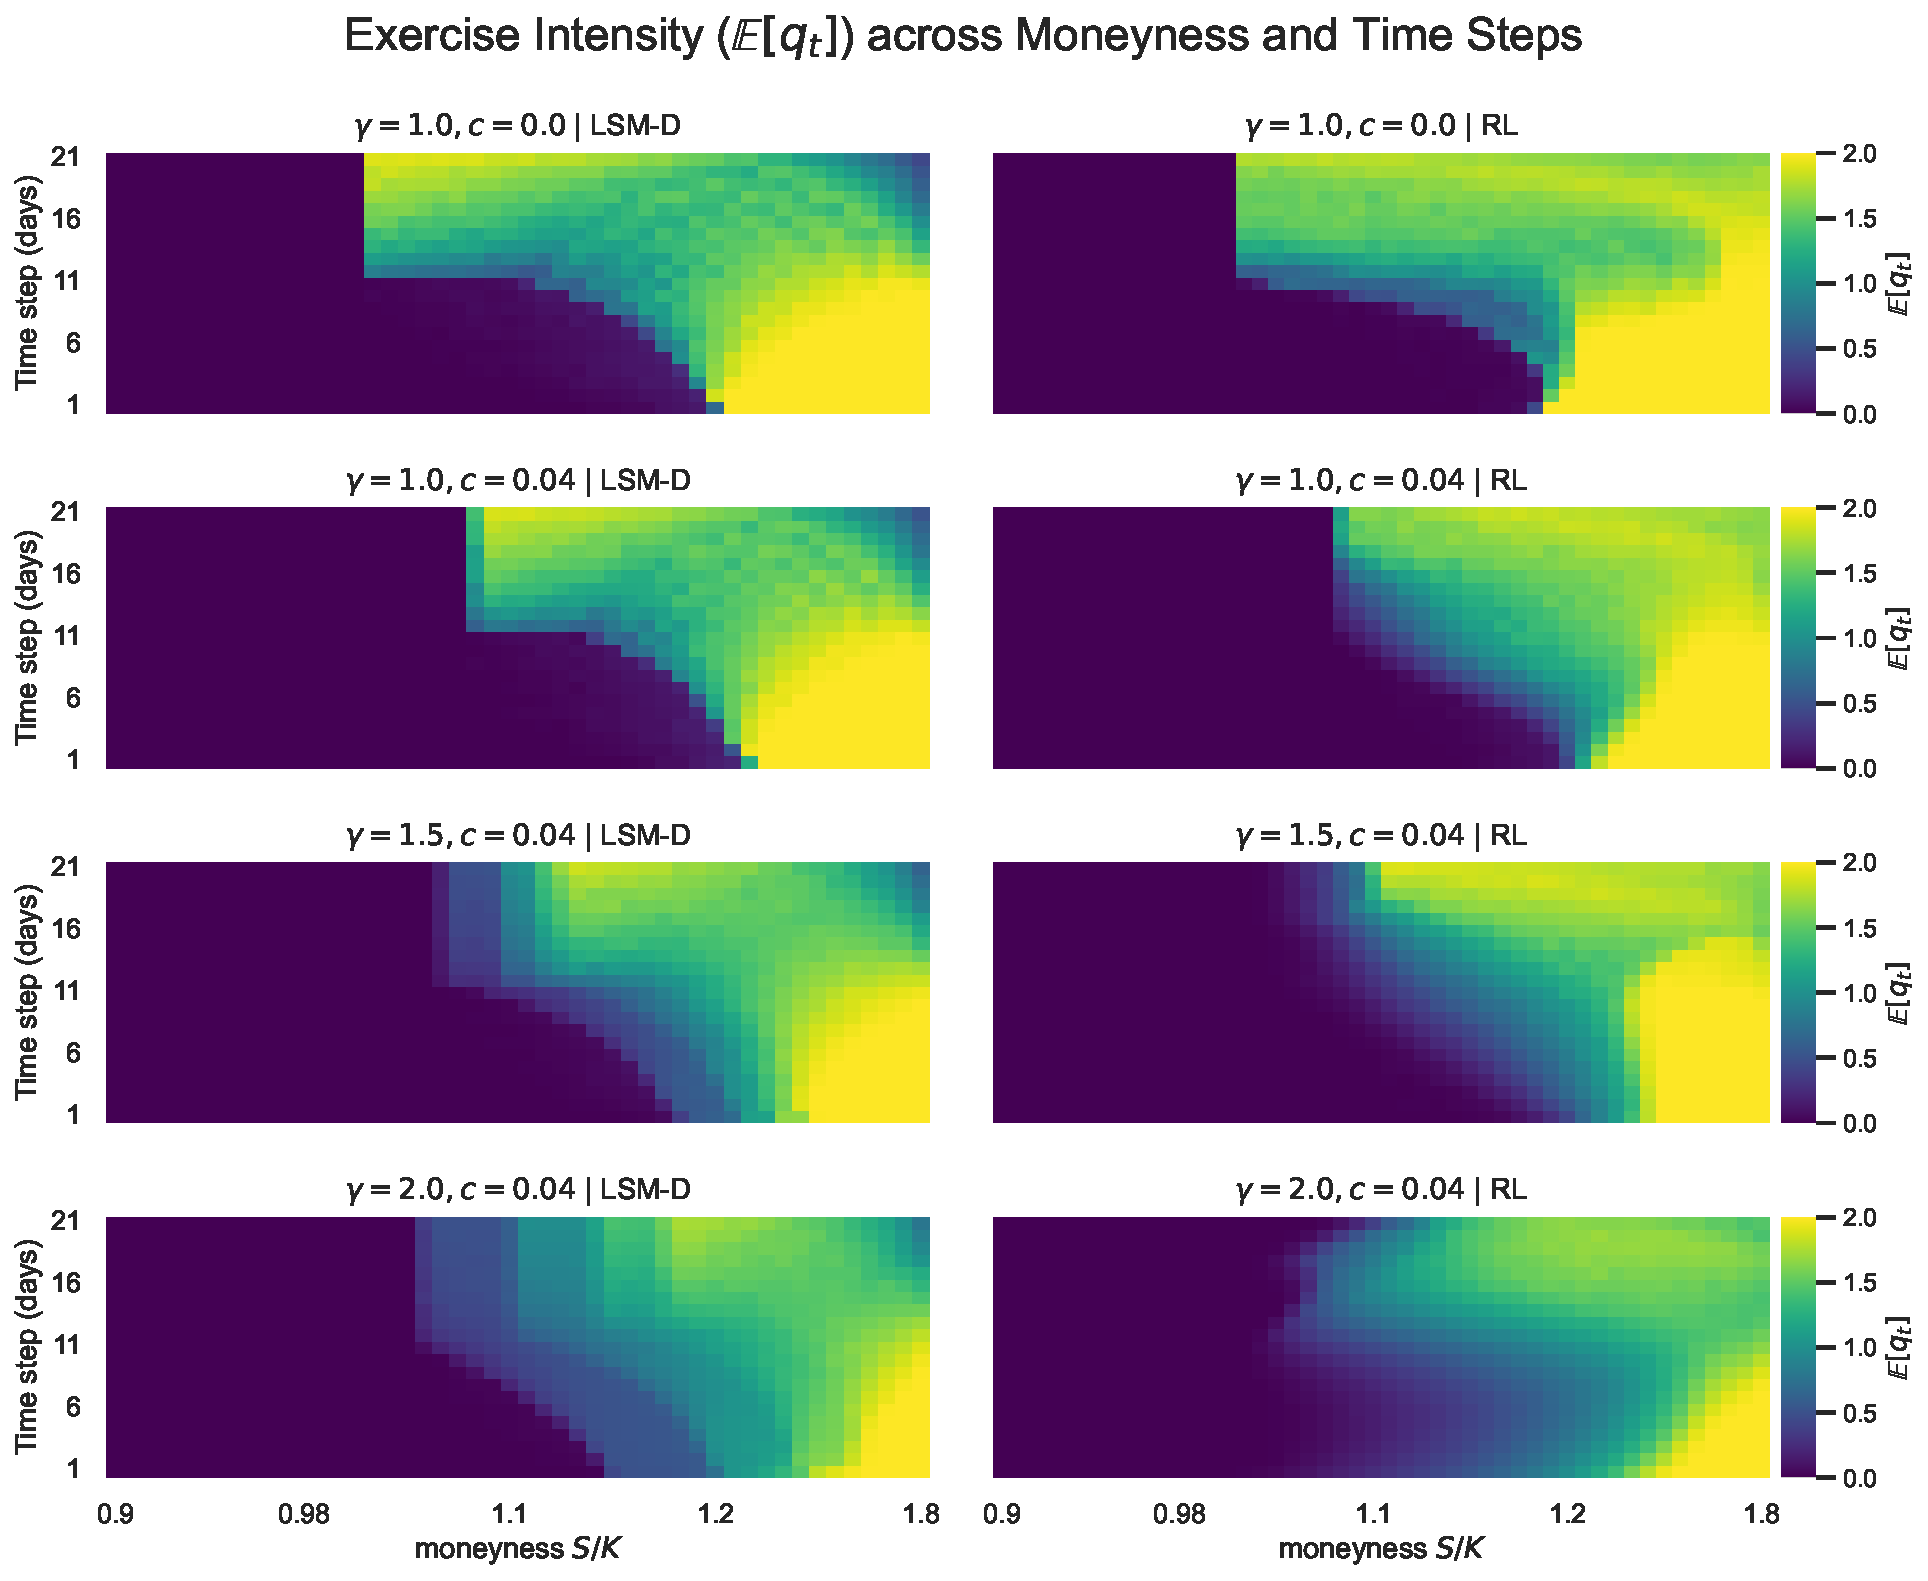
\includegraphics[width=\textwidth]{../figs/convex_costs_0p04/hist_exercise.pdf}
    \caption{\textcolor{green}{Expected exercise quantity $\mathbb{E}[q_t]$ under the continuous DRL policy and the \textcolor{revisionbrown}{discretized-action ($M = 5$)} LSM baseline for a cost coefficient $c=0.04$ and varying convexity parameters $\gamma_c \in \{1.0, 1.5, 2.0, 3.0\}$. The heatmap displays the average fraction of capacity exercised at each available time step (measured in days to contract maturity) as a function of moneyness ($S/K$). Under linear costs ($\gamma_c = 1$), both policies exhibit bang-bang behavior at high moneyness. \textcolor{revisionbrown}{As convexity increases, both the actor--critic network and the LSM baseline transition to graduated exercise quantities, with the RL agent producing smoother intensity gradients across the moneyness--time surface.}}}
    \label{fig:exercise_heatmap}
\end{figure*}

\begin{figure*}[!ht]
    \centering
    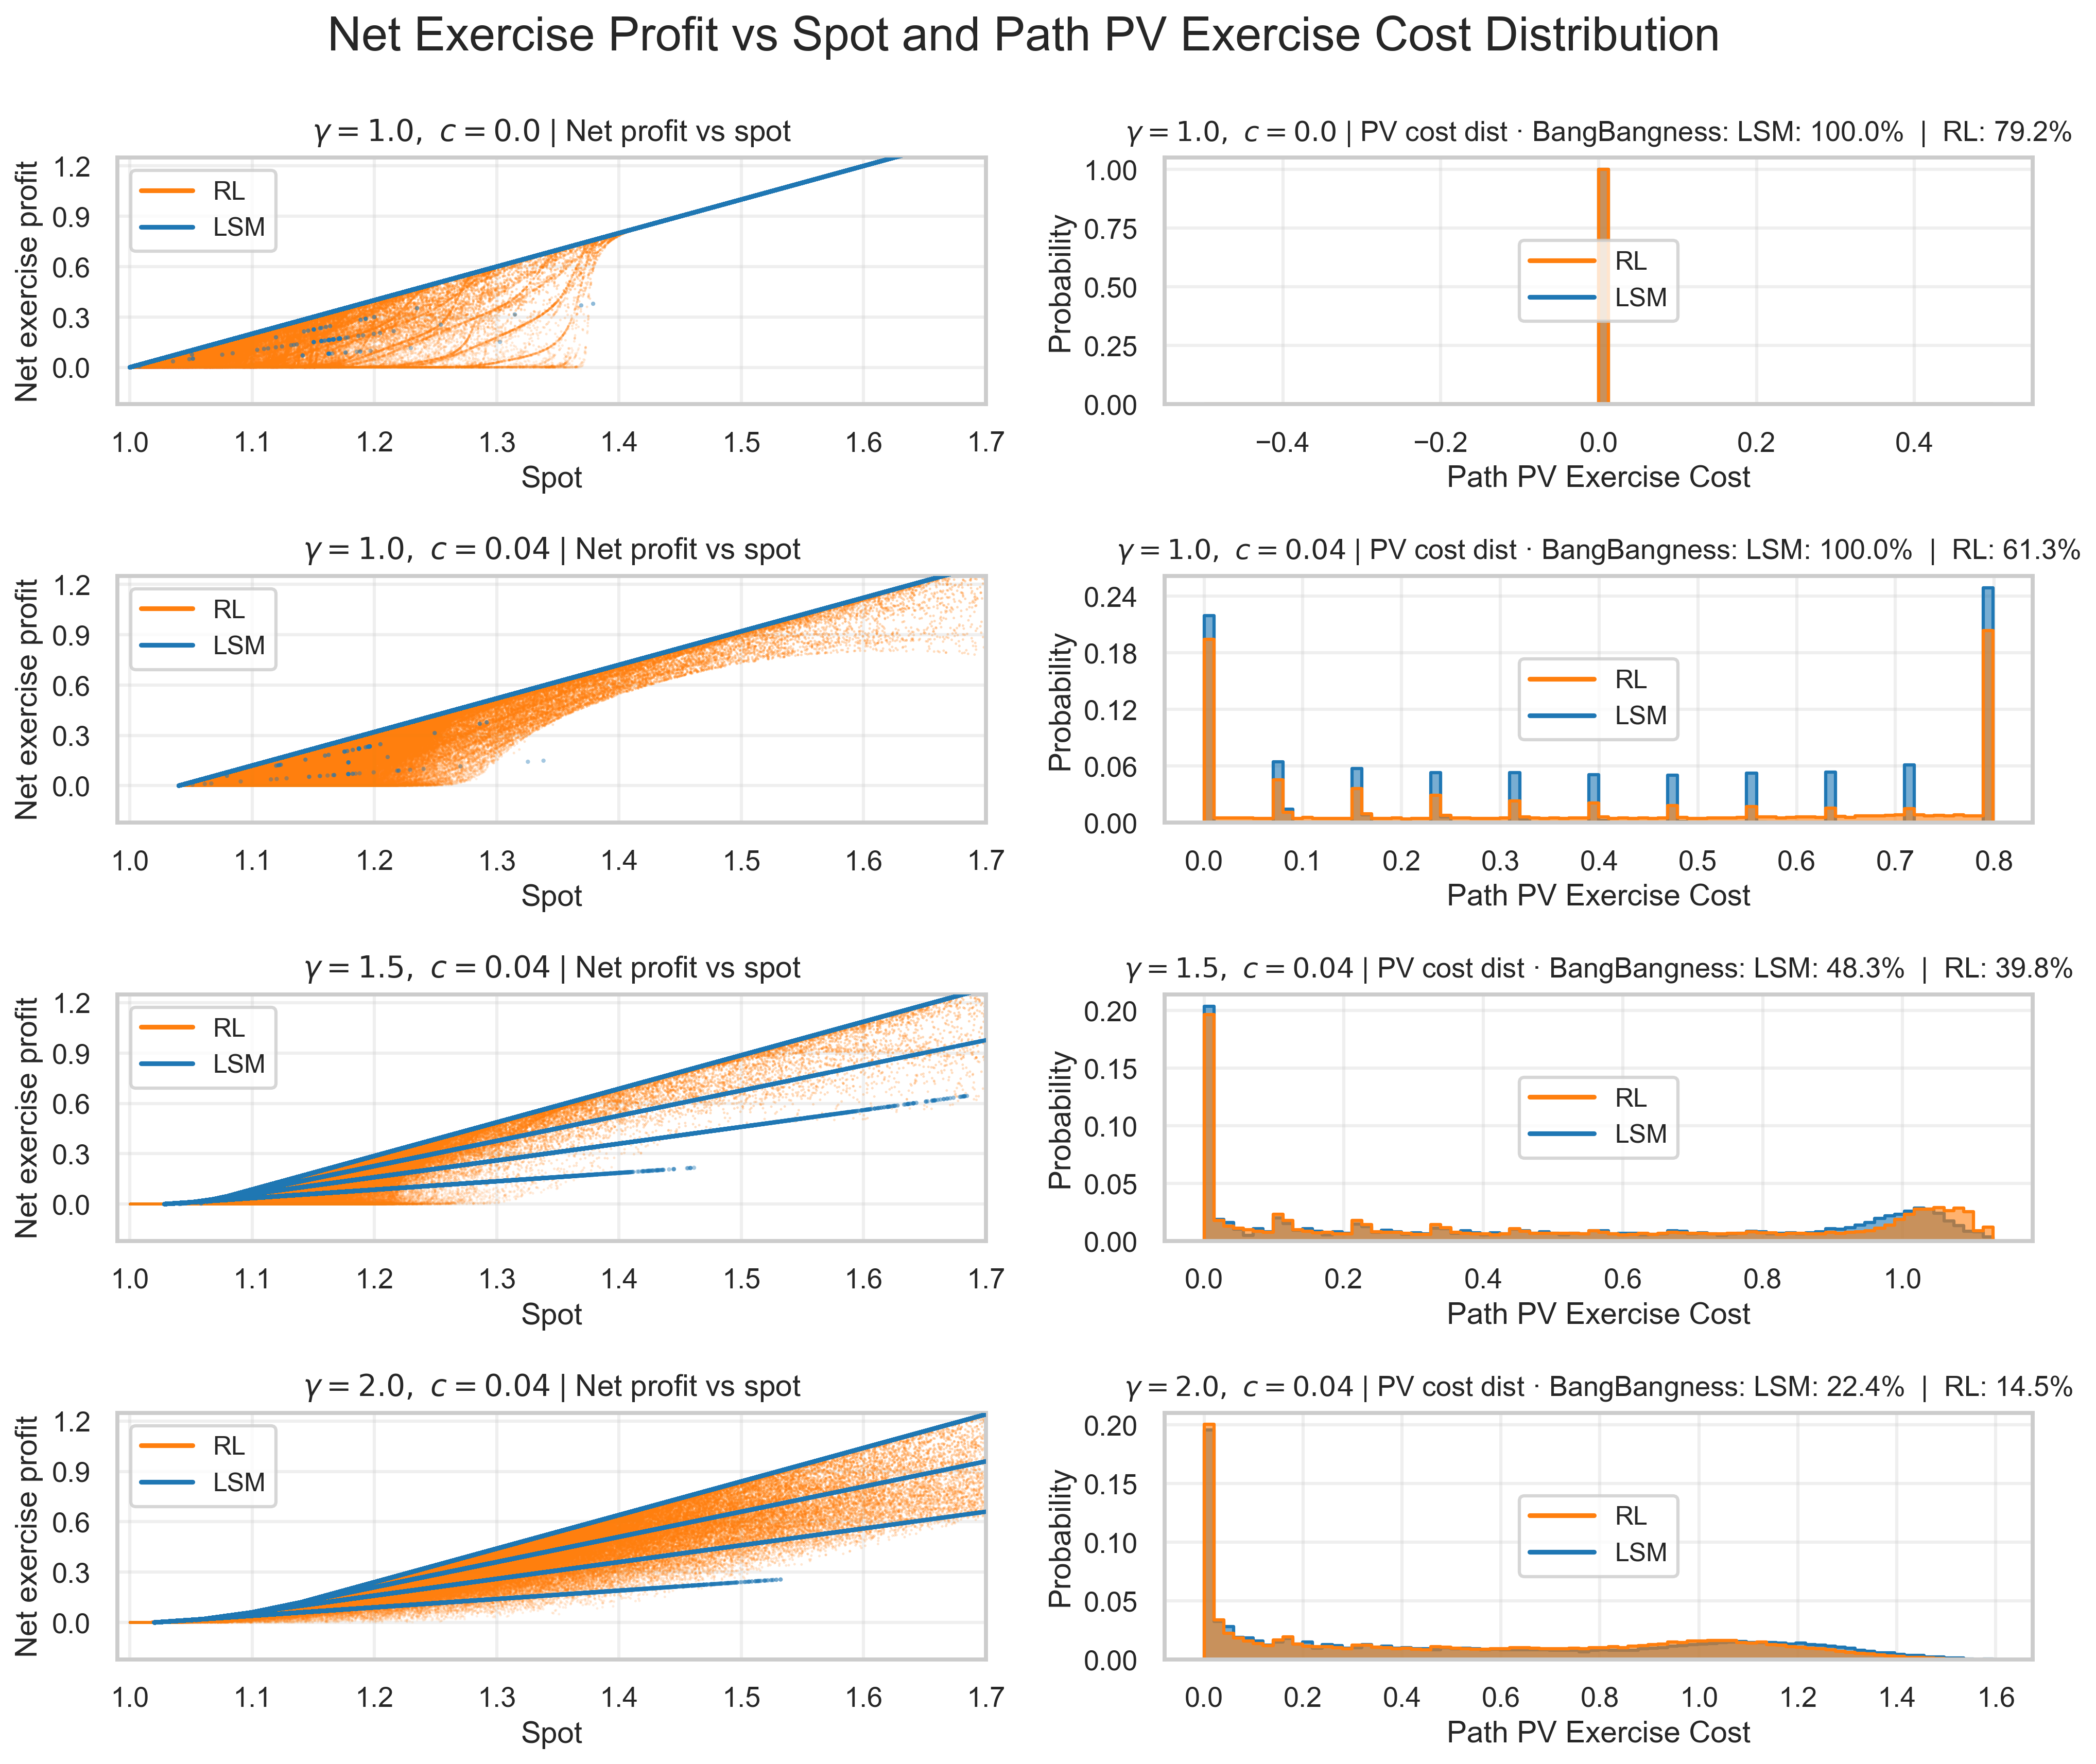
\includegraphics[width=\textwidth]{../figs/convex_costs_0p04/spot_income_pv_hist.png}
    \caption{\textcolor{green}{Net exercise profit versus spot price (left column) and path-level PV exercise cost distribution (right column) for linear ($\gamma_c=1.0$) and convex ($\gamma_c \in \{1.5, 2.0\}$) costs at $c=0.04$. The left column scatters the non-discounted one-step net exercise profit, $q_t(S_t-K)^+ - c q_t^{\gamma_c}$, over the spot price for decisions where exercising full capacity is feasible, with the LSM points overlaid as blue outlines so both methods remain visible in the same region. Under linear costs, \textcolor{revisionbrown}{both the LSM and RL policies tightly track the same bang-bang boundary}. However, under convexity, \textcolor{revisionbrown}{both methods transition to graduated exercise; the continuous RL agent produces denser scatter below the bang-bang frontier, while the discretized-action ($M = 5$) LSM baseline selects from five volume levels}. The right column displays the distribution of total discounted exercise costs per path and tracks the Bang-Bangness metric $B$. \textcolor{revisionbrown}{As convexity grows, both methods reduce their Bang-Bangness and shift towards more distributed exercise strategies.}}}
    \label{fig:spot_income_pv_hist}
\end{figure*}

\subsection{\textcolor{green}{Analysis of Exercise Behavior}}
\label{sec:exercise_behavior}

\textcolor{green}{To quantify the degree to which a learned policy adheres to the all-or-nothing exercise decisions typical of linear cost structures, we introduce the \emph{Bang-Bangness} metric $B$. We define $B$ as the proportion of feasible full-capacity exercises that actually hit the maximum allowable quantity. Specifically, over the subset of steps where the remaining capacity is at least the maximum single-step limit ($Q_{\max} - Q_i \ge q_{\max}$) and the agent chooses to exercise a strictly positive amount ($q_t > 0$), the metric is defined via the Hit-Ratio:}
\begin{equation}
    B = \mathbb{P}\left( \frac{q_t}{q_{\max}} \ge 0.95 \;\middle|\; Q_{\max} - Q_i \ge q_{\max},\, q_t > 0 \right).
\end{equation}
\textcolor{green}{A \textcolor{revisionbrown}{bang-bang} policy yields $B=100\%$, while a completely uniform random exercise decision over $(0, q_{\max}]$ would yield an expected baseline of $B \approx 5\%$.}

\begin{figure}
    \centering
    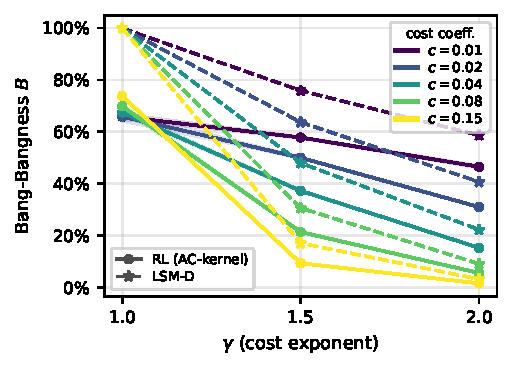
\includegraphics[width=\columnwidth]{../figs/convex_costs_0p04/bang_bangness_rl.pdf}
    \caption{\textcolor{green}{The Bang-Bangness metric $B$ across five representative cost regimes ($c \in \{0.01, 0.02, 0.04, 0.08, 0.15\}$) and convexities for the RL and LSM agents. \textcolor{revisionbrown}{Both methods systematically decrease the proportion of maximum-capacity exercises as the cost exponent ($\gamma$) grows, confirming that the learned policies adapt to convex penalties by distributing exercise across multiple quantities.}}}
    \label{fig:bang_bangness_trend}
\end{figure}

\textcolor{green}{Figure~\ref{fig:spot_income_pv_hist} provides a microscopic view of the exercise behavior \textcolor{revisionbrown}{under both methods}. The left column scatters the non-discounted one-step net exercise profit against the underlying spot price. When $c > 0$ and costs are linear ($\gamma_c=1.0$), \textcolor{revisionbrown}{both the RL agent and the discretized-action LSM baseline produce near-identical exercise boundaries, confirming that bang-bang exercise is optimal under linear costs}.}

\textcolor{green}{However, under convex costs ($\gamma_c \in \{1.5, 2.0\}$), a dense region of profitable partial exercise emerges beneath the strict bang-bang frontier. \textcolor{revisionbrown}{Both methods exploit this region: the LSM baseline selects from five discrete volume levels while the actor--critic agent continuously modulates its exercise quantity, producing a denser scatter of intermediate exercise decisions.}}

\textcolor{green}{This behavioral shift is corroborated by the right column of Figure~\ref{fig:spot_income_pv_hist}, which depicts the distribution of the path-level present value of exercise costs. At $\gamma_c=1.0$, the RL agent exhibits high Bang-Bangness (\textcolor{revisionorange}{$B \approx 66\%$}) and its cost distribution closely tracks that of the LSM baseline. As the cost exponent increases to $\gamma_c = 2.0$, \textcolor{revisionbrown}{both methods show markedly reduced Bang-Bangness---the RL agent decays to $B \approx 21\%$ while the LSM baseline reaches a similar $B \approx 22\%$---reflecting their shared adaptation to convex penalties through graduated exercise}.}

\subsection{Discussion}

\textcolor{revisionbrown}{Three qualitative patterns stand out in Table~\ref{tab:results} and Figures~\ref{fig:exercise_heatmap} and~\ref{fig:spot_income_pv_hist}.}
\begin{enumerate}
    \item \textcolor{revisionbrown}{\textbf{Baseline competitiveness.} Across most of the $(c, \gamma_c)$ grid, the discretized-action LSM baseline is competitive with or slightly exceeds the actor--critic method. The typical deficit is $1$--$2\%$, consistent with the remaining gap between a five-level action grid and a truly continuous policy.}
    \item \textcolor{revisionbrown}{\textbf{Near-parity under strong convexity.} For $\gamma_c \ge 2$ with moderate cost coefficients, the gap between the two methods narrows substantially. This is the regime where both methods benefit from interior exercise and neither has a decisive structural advantage.}
    \item \textcolor{revisionbrown}{\textbf{RL advantage at extremes.} For the three configurations with both high cost coefficient and high convexity exponent ($c \ge 0.05$, $\gamma_c \ge 2$), the actor--critic method marginally outperforms the LSM baseline. The continuous action space may help in these highly non-linear regimes where five discrete levels provide coarser cost-quantity trade-offs.}
\end{enumerate}

\textcolor{revisionbrown}{These results support a nuanced interpretation: the discretized-action LSM baseline is a strong classical comparator that captures most of the value from interior exercise. The actor--critic approach does not systematically dominate but rather provides a complementary methodology whose main advantages lie in avoiding explicit state-space discretisation and scaling more naturally to complex contract features.}

% P2-8: Address the weak-baseline critique explicitly.
\paragraph{Caveat: comparator strength.}
\textcolor{revisionbrown}{A crucial caveat is that the $M\!=\!5$ LSM baseline, while substantially stronger than the classical bang-bang ($M\!=\!2$) variant used in earlier drafts, is still limited by its finite action grid and polynomial continuation-value approximation. Two sources of residual suboptimality remain: (i)~the five-level grid cannot represent exercise quantities between grid points, and (ii)~the degree-$2$ Chebyshev basis may miss non-linear continuation-value features in extreme cost regimes. Conversely, the actor--critic method faces its own approximation limitations through finite training, seed sensitivity, and the implicit bias of neural-network function approximation.}
Additionally, the absence of an upper bound (e.g.\ a dual martingale bound in the spirit of \citealt{andersen2004primal}) means we cannot certify how close either method is to the true option value.

\textcolor{green}{From a practical optimisation perspective, two engineering gaps remain. First, although the focal robustness study shows very low seed dispersion under the final evaluation protocol, the longer-term goal is a training procedure that is reliable enough that one seed is effectively sufficient in routine use, and for which additional training episodes improve the policy or at least do not degrade it. Second, the current CPU implementation is still far from production-grade throughput: substantial software and hardware optimisation, especially GPU-oriented batching and parallelisation, will be required before this approach can be deployed at much larger scale. Relative to earlier DRL derivatives work, however, the present pipeline is already materially more robust and more computationally disciplined; compare the stronger seed sensitivity and training inefficiency documented for American-option hedging in \citealt{tsoskounoglou2025higherorder}.}

\subsection{\textcolor{revisionorange}{Seed Robustness}}
\label{sec:seed_robustness}

\textcolor{revisionorange}{To assess the sensitivity of the learned price to the training random seed, we conduct a focal robustness study for the representative configuration $c = 0.04$, $\gamma_c = 2$. In addition to the three seeds used in Table~\ref{tab:results}, twelve further seeds (14--25) are trained with identical hyperparameters and evaluated on the common test set. Figure~\ref{fig:seed_robustness} shows the resulting distribution of 15 test-set prices.}

\begin{figure}
    \centering
    \IfFileExists{../figs/convex_costs_0p04/seed_robustness.pdf}{%
        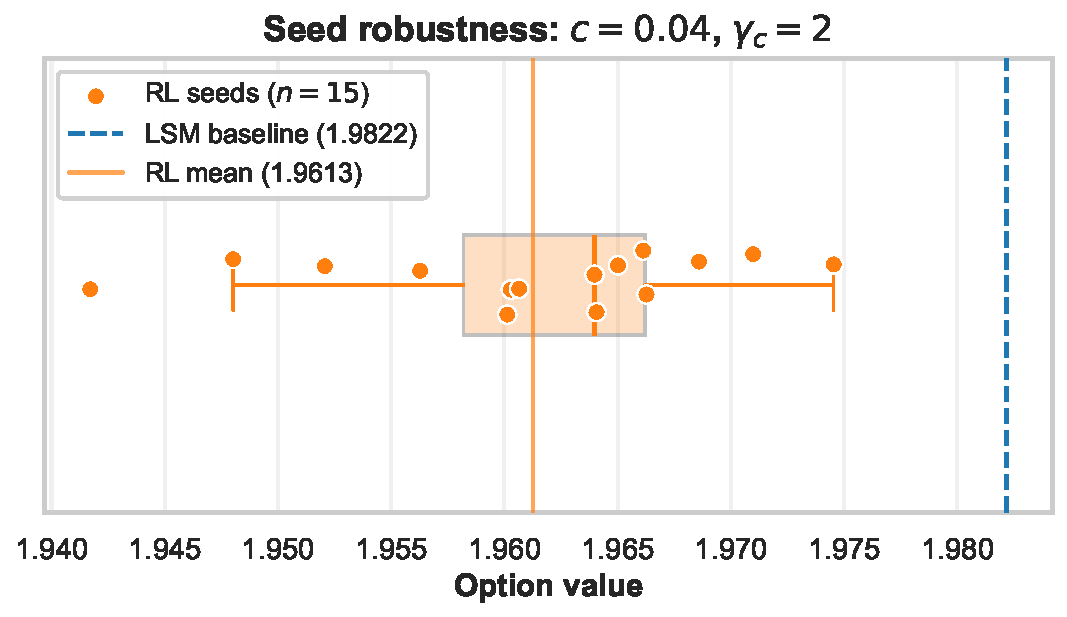
\includegraphics[width=\columnwidth]{../figs/convex_costs_0p04/seed_robustness.pdf}%
    }{%
        \framebox[\columnwidth]{\parbox{0.9\columnwidth}{\centering\vspace{2em}\textit{Figure placeholder --- run focal training and generate figure.}\vspace{2em}}}%
    }
    \caption{\textcolor{revisionorange}{Distribution of RL option values across 15 independent training seeds ($c = 0.04$, $\gamma_c = 2$). The vertical dashed line indicates the \textcolor{revisionbrown}{discretized-action ($M = 5$)} LSM baseline. \textcolor{revisionbrown}{The narrow spread confirms consistent training, although the distribution sits slightly below the LSM baseline for this configuration.}}}
    \label{fig:seed_robustness}
\end{figure}

\textcolor{revisionorange}{The inter-seed standard deviation is $0.009$ (coefficient of variation $0.45\%$), confirming that the training procedure yields consistent pricing estimates across random initialisations. \textcolor{revisionbrown}{For this configuration, all 15 seeds produce test-set values within $2\%$ of the discretized-action LSM baseline (range: $-2.0\%$ to $-0.4\%$). The tight clustering demonstrates that while the actor--critic method does not surpass the upgraded LSM baseline here, its cross-seed variability is small enough that the difference is economically modest.}}

\subsection{Computational Efficiency}

Training for $32{,}768$ episodes requires approximately $2$--$3$ hours on a $4$-core CPU. Once trained, the policy is cheap to evaluate: on the archived experiments, valuing $65{,}536$ held-out paths took less than $10$ seconds. The computational burden is thus shifted from repeated backward induction to one-off policy training.

\section{Conclusion}
\label{sec:conclusion}

We have formulated electricity swing-option valuation under the HHK jump-diffusion model as a finite-horizon stochastic control problem and approximated its solution with a deterministic actor--critic method. The central modelling device is a profitability-gated actor that clips candidate exercises to quantities with non-negative immediate payoff while preserving a usable gradient signal through a straight-through estimator.

\textcolor{revisionbrown}{The numerical results indicate that a discretized-action ($M = 5$) LSM baseline is a strong classical comparator: it generally matches or slightly exceeds the actor--critic method across the tested cost configurations. The actor--critic approach remains within $1$--$2\%$ of the LSM baseline in most cases and marginally outperforms it in a small number of configurations with high cost convexity, where the continuous action space may provide finer exercise resolution.} The present experiments focus on optional exercise with a cumulative cap and no active refraction lag.

\textcolor{revisionbrown}{Several directions for future work are worth highlighting. First, constructing dual upper bounds---for example, via an adaptation of the Andersen--Broadie or Haugh--Kogan methodology to the swing setting---would provide an independent assessment of how close either method is to the true optimum. Second, extending the LSM baseline to a finer action grid or a randomised basis-selection scheme could further narrow the remaining gap. Third, extending the contract specification to include mandatory take obligations, non-trivial refraction lags, and calibration to observed forward and option data would broaden the practical relevance of both approaches.}

\section*{Acknowledgement}

The authors gratefully acknowledge financial support from the Amsterdam University Fund through the AUF Impact Call (Fall 2024), together with additional support from the AI4FinTech initiative at the University of Amsterdam.

\bibliographystyle{model1-num-names}
\bibliography{Bibliography}

\end{document}